
\documentclass[reqno,11pt]{amsart}

%\usepackage{color,graphicx}
%\usepackage{mathrsfs,amsbsy}
\usepackage{amssymb}
\usepackage{amsmath}
\usepackage{amsfonts}
\usepackage{bm}
\usepackage{graphicx}
\usepackage{amsthm}
\usepackage{enumerate}
\usepackage[mathscr]{eucal}
\usepackage{float}
\usepackage{mathrsfs}
\usepackage{multicol}
\usepackage[all,pdf]{xy}
\usepackage[a4paper,left=3cm,right=3cm]{geometry}

%\usepackage[notcite,notref]{showkeys}

% showkeys  make label explicit on the paper

\makeatletter
\@namedef{subjclassname@2010}{%
  \textup{2010} Mathematics Subject Classification}
\makeatother

\numberwithin{equation}{section}

\theoremstyle{plain}
\newtheorem{theorem}{Theorem}[section]
\newtheorem{lemma}[theorem]{Lemma}
\newtheorem{proposition}[theorem]{Proposition}
\newtheorem{corollary}[theorem]{Corollary}
\newtheorem{claim}[theorem]{Claim}
\newtheorem{defn}[theorem]{Definition}
\newtheorem{ques}[theorem]{Question}
\newtheorem*{fact}{Facts}
\newtheorem{eg}[theorem]{Example}

\theoremstyle{plain}
\newtheorem{thmsub}{Theorem}[subsection]
\newtheorem{lemmasub}[thmsub]{Lemma}
\newtheorem{corollarysub}[thmsub]{Corollary}
\newtheorem{propositionsub}[thmsub]{Proposition}
\newtheorem{defnsub}[thmsub]{Definition}

\numberwithin{equation}{section}


\theoremstyle{remark}

\newtheorem{remark}[theorem]{Remark}
\newtheorem{remarks}{Remarks}
\newcommand*\widebar[1]{%
	\hbox{%
		\vbox{%
			\hrule height 0.5pt % The actual bar
			\kern0.6ex%         % Distance between bar and symbol
			\hbox{%
				\kern 0em%      % Shortening on the left side
				\ensuremath{#1}%
				\kern 0em%      % Shortening on the right side
			}%
		}%
	}%
}
\renewcommand\thefootnote{\fnsymbol{footnote}}
%dont use number as footnote symbol, use this command to change

\DeclareMathOperator{\supp}{supp}
\DeclareMathOperator{\dist}{dist}
\DeclareMathOperator{\vol}{vol}
\DeclareMathOperator{\diag}{diag}
\DeclareMathOperator{\tr}{tr}

\begin{document}
\date{}

\title
{The Equivariant Tubular Neighborhood Theorem}


\author{Xiaoxiang Zhou}
\address{School of Mathematical Sciences\\
University of Science and Technology of China\\
Hefei, 230026\\ P.R. China\\} 
\email{email:xx352229@mail.ustc.edu.cn}





\begin{abstract}
The equivariant tubular neighborhood theorem is a interesting generalization of the tubular neighborhood theorem, which describes the group action near an invariant embedding submanifold. I will introduce the necessary tools and prove the theorem from the simplest case to the most general case.
\end{abstract}



\maketitle
%%%%%%%%%%%%%%%%%%%%%%%%%%%%%%%%%%%%%%%%%%%%%%%%%%%%%%%%%%%%%%%%%%%%%%%%%%%%%%%%%%%%%%%%%%%%%


\section{the Statement of the Theorem}
	
In Prof.Wang's lecture notes \cite{ZW1} (Lecture 10, Theorem 2.2) we have seen the following theorem:
\begin{theorem}\label{thm:main}
	(Tubular Neighborhood Theorem). Let $N \subseteq M$ be a smooth embedding submanifold.
	Then there exists a \textbf{diffeomorphism} from an open neighborhood of $N$ in the normal bundle $\mu_N$ of $N$ onto an open neighborhood of $N$ in $M$.
\end{theorem}
  Now we want to add group action $\tau$ of $G$ on $M$ which maps points in $N$ to points in $N$. We want to find out
  \begin{center}
  	\fbox{\textbf{Question:} What does the group action looks like ``near" $N$?}
  \end{center} 
\begin{eg}
	Consider the group $G=S^1$ acts on $M=S^2$ by rotation
	\begin{equation*}
	\begin{aligned}
		S^1 &\text{ \rotatebox[origin=c]{270}{$\circlearrowleft$} }\hspace{1.5cm} S^2\\
		\theta\; &\mapsto [(\varphi,h)\mapsto(\varphi+\theta,h)]
	\end{aligned}
	\end{equation*}
	
Denote $N:=\{(\varphi,0) \in S^2\} \cong S^1$ is the embedding submanifold of $S^2$, which is $G$-invariant under the action $\tau$, i.e.
$\tau (N) \subseteq N$.
Denote $U=\left\{(\varphi,h)\in S^2 \big| |h| < 1/2\right\}$ to be the tubular neighbourhood of $N$, $\mu_N$ to be the normal bundle of $N$ in $M$, we have
	\begin{equation*}
	\begin{aligned}
	\Phi:\mu_N \cong N \times \mathbb{R} &\longrightarrow \hspace{0.8cm} U\\
	(\theta\,,\,r)\; &\;\mapsto (\theta,\frac{r}{2\sqrt{1+r^2}})
	\end{aligned}
	\end{equation*}
	Moreover, this tubular neighbourhood is compatible with the group action $\tau$, i.e. $G \cdot U \subseteq U$ and the diagram commutes:
\begin{equation*}
	\SelectTips{eu}{12}
		\xymatrix{
		U\ar[r]_{\sim}^{\Phi}\ar[d]_{\tau_g} & \mu_N\ar[r]^{\pi}\ar[d]^{(\tau_g)_*} & N\ar[d]^{\tau_g} \\
		U\ar[r]_{\sim}^{\Phi} & \mu_N\ar[r]^{\pi} & N	
	}
\end{equation*}
\end{eg}
\begin{remark}
	This is generally NOT TRUE if we take $U$ to be a non-regular shapes or $\Phi$ not so good identified. However, as the following theorem states, If the $G$-action is good enough, then one can always find a GOOD tubular neighbourhood with a GREAT identification $\Phi$.
\end{remark}
\begin{figure}[th]
	\begin{minipage}[t]{.32\textwidth}
		\centering
		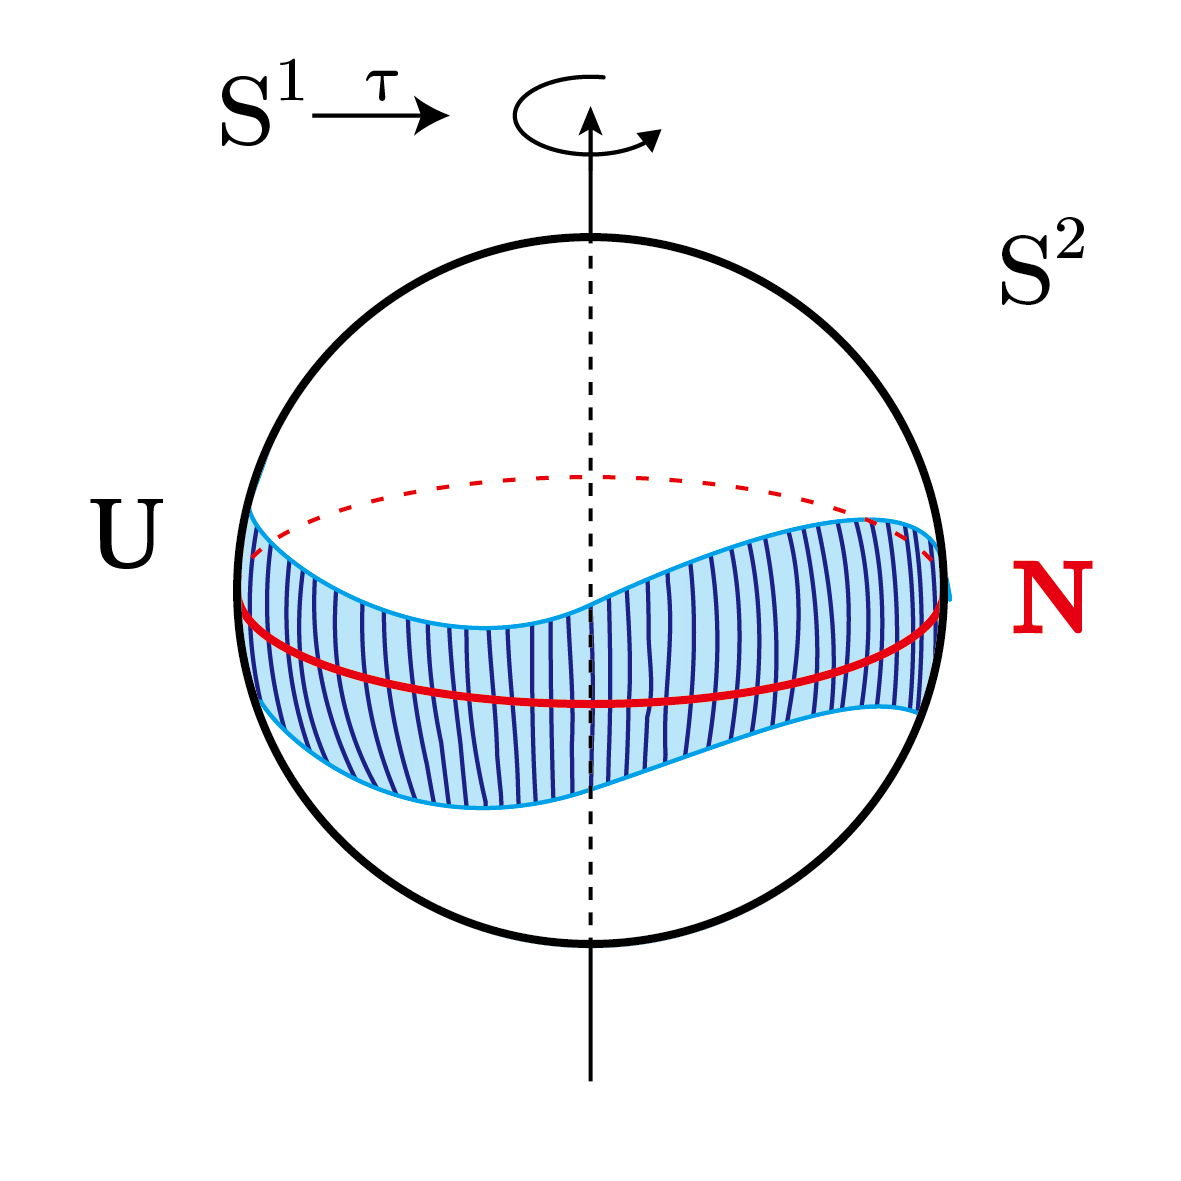
\includegraphics[width=\textwidth]{figures/figure6-01.png}\\
		non-regular shape
		
		\label{fig1}
	\end{minipage}
	\begin{minipage}[t]{.32\textwidth}
		\centering
		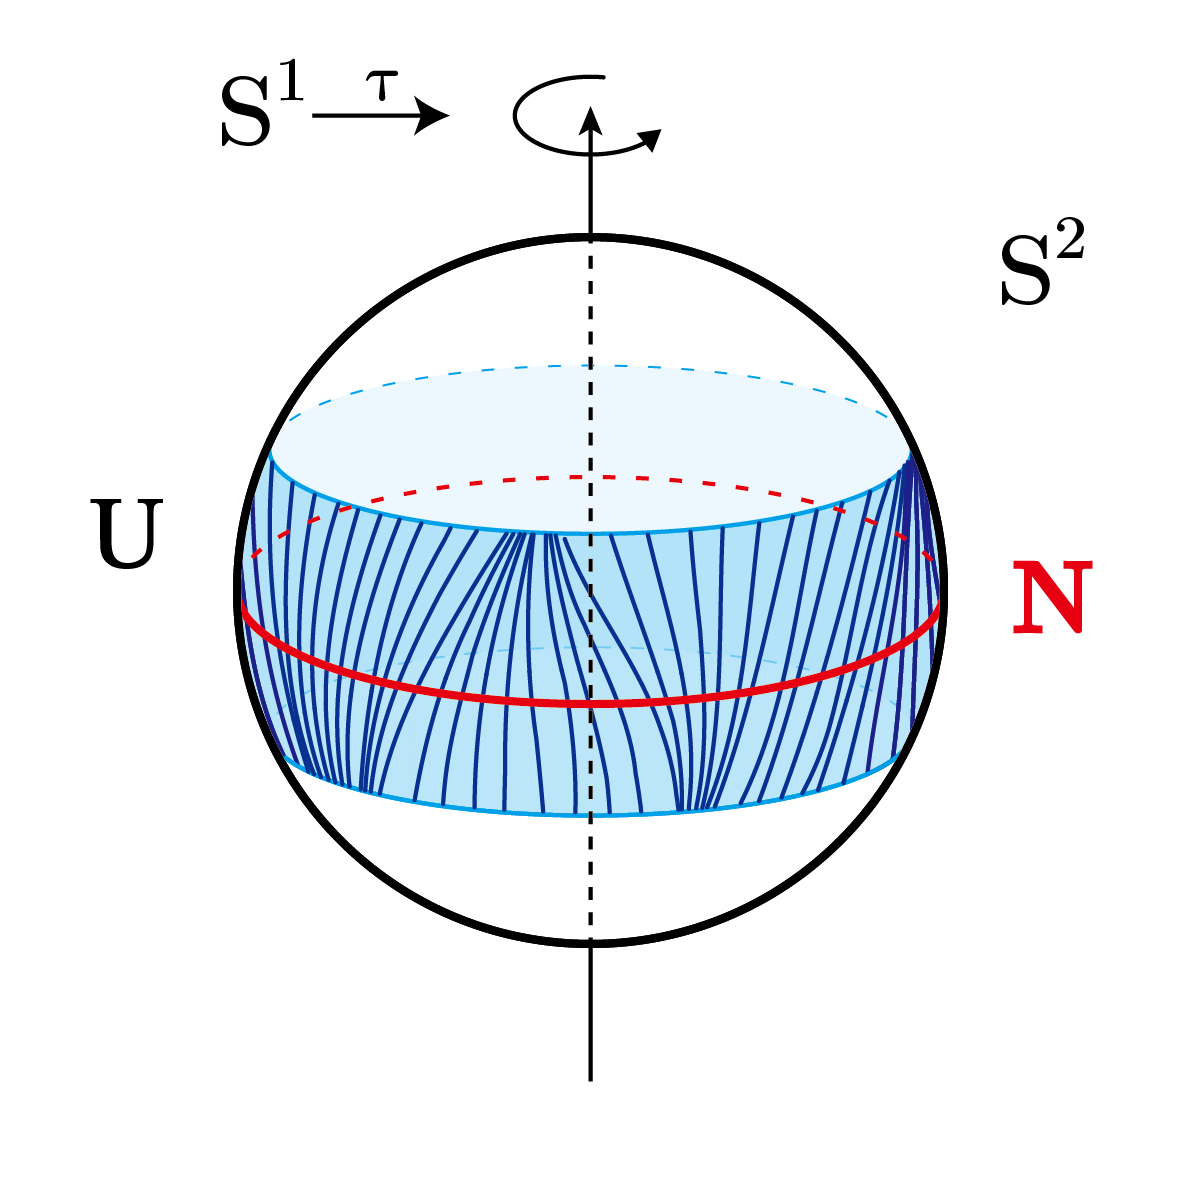
\includegraphics[width=1\textwidth]{figures/figure2-01.png}\\
		bad identification
		\label{fig2}
	\end{minipage}
	\begin{minipage}[t]{.32\textwidth}
		\centering
		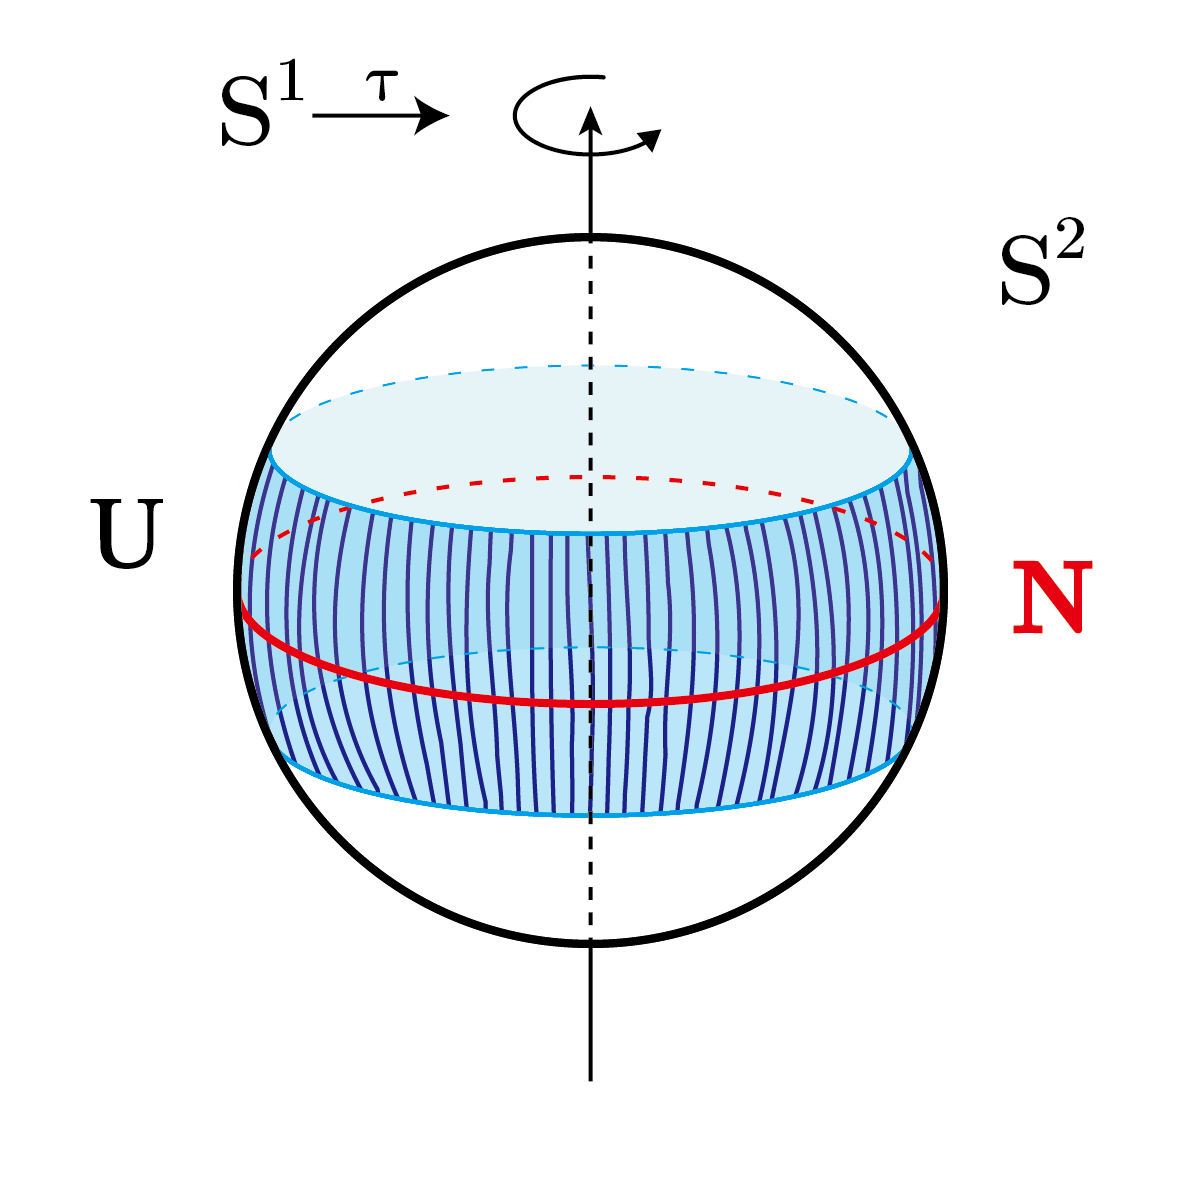
\includegraphics[width=\textwidth]{figures/figure7-01.png}\\
		good tubular neighbourhood
		\label{fig3}
	\end{minipage}
\caption{}
\end{figure}
\begin{defn}
	Let $G$ be a Lie group acting on the manifold $X$ and $Y$. We say that the function $f:X\rightarrow Y$ is a \textbf{G-equivariant map} if the function commutes with the action of the group, i.e. the following diagram commutes:
	\begin{equation*}
		\SelectTips{eu}{12}
	\xymatrix{
		X\ar[r]^{\tau_g}\ar[d]_{f} & X\ar[d]^{f} \\
		Y\ar[r]^{\tilde{\tau}_g} & Y
	}
	\end{equation*}
\end{defn}
\begin{theorem}(The Equivariant Tubular Neighborhood Theorem)
	 Suppose a compact Lie group $G$
	acts on a smooth manifold $M$ smoothly. Then for any $G$-invariant smooth submanifold $N$
	of $M$, there exists a \textbf{G-equivariant diffeomorphism} from the normal bundle $\mu_N$ of $N$ to a
	neighborhood of $N$ in $M$, which is the identity map when restricted to $N$.
	\begin{equation*}
		\SelectTips{eu}{12}
	\xymatrix@R=0.4cm@C=0.45cm{
		&&U\ar[rrrr]^{\tau_g}&&&&U\\
		\mu_N\ar[rrrr]^(0.6){(\tau_g)_*}&&&&\mu_N&&\\
		&&&&&&\\
		&N\ar[rrrr]^{\tau_g}&&&&N&
		\ar"2,1";"1,3"^{\Phi}
		\ar"2,1";"4,2"_{\pi}
		\ar"1,3";"4,2"^(0.55){\tilde{\pi}}|(0.38)\hole
		\ar"2,5";"1,7"^(0.42){\Phi}
		\ar"2,5";"4,6"_{\pi}
		\ar"1,7";"4,6"^{\tilde{\pi}}		
	}
	\end{equation*}
\end{theorem}
\begin{figure}[th]
		\centering
		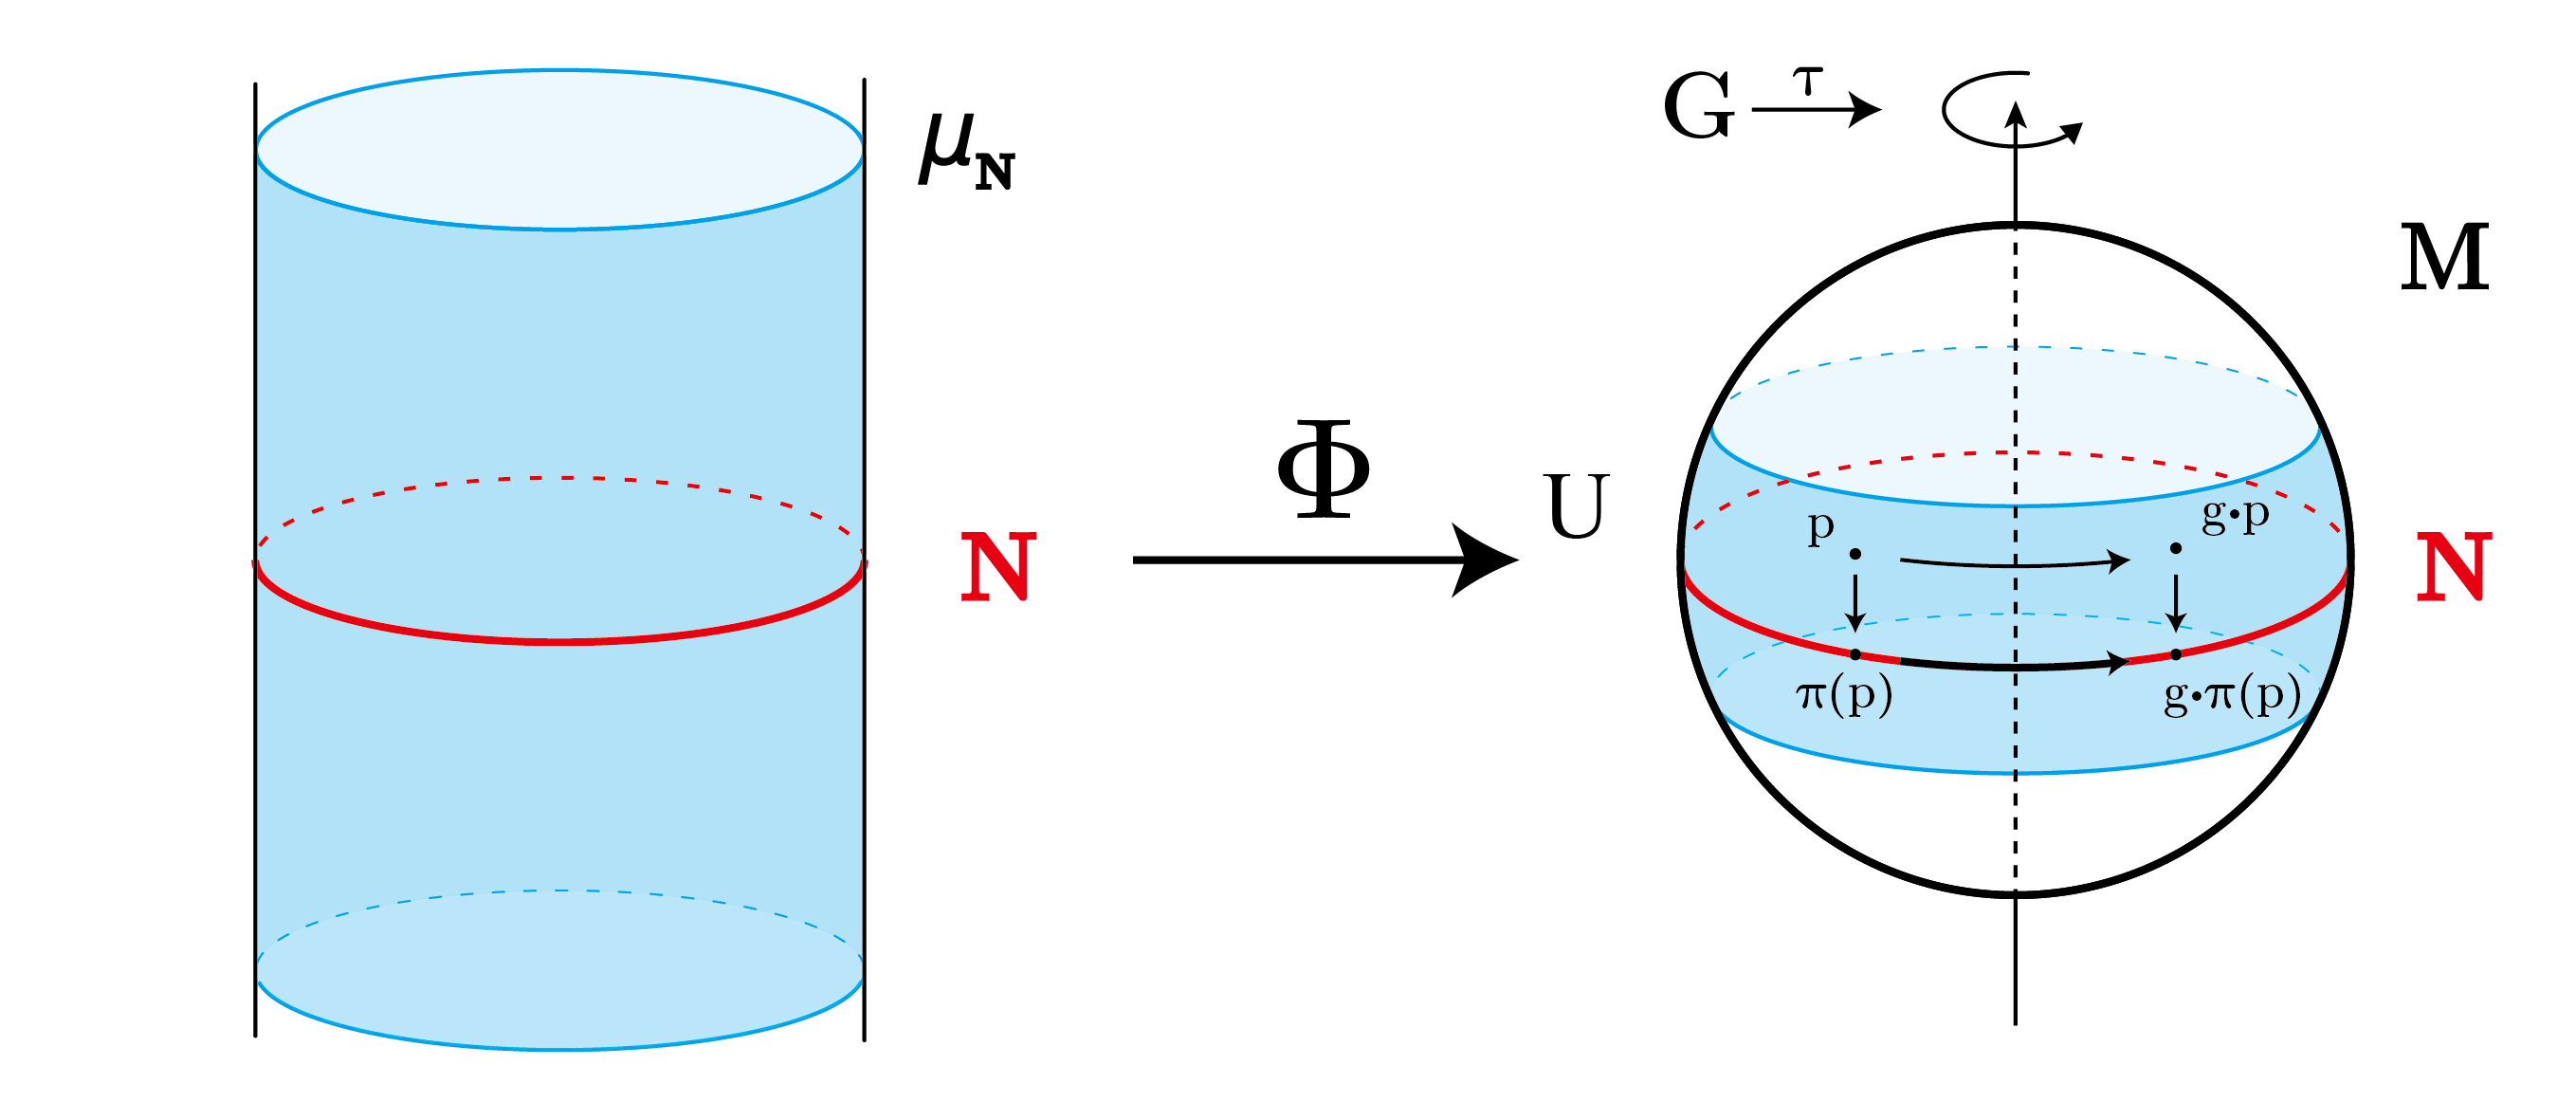
\includegraphics[width=\textwidth]{figures/final2-01.png}\\
		\caption{}
		\label{fig4}
\end{figure}
\begin{remark}\ 
	\begin{itemize}
		\item When $G$ is a finite group, $G$ is automatically a compact. We will first prove the case when $G$ is a finite group, then generalize it into the most general case.
		\item If $G$ is not compact, the theorem still holds if we assume the $G$-action is \textbf{proper},i.e. the map
		\begin{equation*}
		\begin{aligned}
			\mathcal{A}:G \times M &\longrightarrow M \times M\\
			(g,m)\;&\mapsto (g \cdot m,m)
		\end{aligned}
		\end{equation*}
	is proper.
	\end{itemize}
\end{remark}
We will need a Riemannian metric on $M$ which is ``compatible with the $G$-action". We will use the Exponential map induced by the metric to construct the diffeomorphism. So let us introduce the following conceptions. 

\section{Riemannian Metric and the Exponential Map}
\subsection{Riemannian Metric}
Notice that the $G$-action on $M$ induces the $G$-action on $TM$:
$$\tau_g:M \longrightarrow M \quad\rightsquigarrow\quad d(\tau_g)_m:T_mM \longrightarrow T_mM$$
and the projection map $\pi:T_mM \rightarrow M$ is a $G$-equivariant map. From now on, if $v \in T_mM$, we will denote $g\cdot v:=d(\tau_g)_m(v)$ to simplify symbolic expressions.
\begin{defn}(Riemannian metric)
	A \textbf{Riemannian metric} on $M$ is a symmetric 2-tensor $g=\left<-,-\right>$ such that for any $m \in M$, $g_m=\left<-,-\right>_m$ is positive definite.
	
	$\left<-,-\right>$ is said to be \textbf{invariant} (with respect to the $G$-action) if
	$$\left<g\cdot v,g\cdot w\right>_{g \cdot m}=\left<v,w\right>_m$$
	for any $v,w \in T_mM$ and $m \in M$. For such a metric, $G$ is said to be act by \textbf{isometries}.
\end{defn}
\begin{remark}
	By problem 10 in PSet6, there exists a Riemannian metric on any smooth manifold $M$.
\end{remark}
When $G$ is finite, we can define a new Riemannian metric on $M$ by
\begin{equation}
\{v,w\}_m=\frac{1}{|G|}\sum_{g \in G} \left<g \cdot v,g\cdot w\right>_{g\cdot m}
\label{eq:riemet}
\end{equation}
Obviously $\{-,-\}_m$ is smooth, linear and symmetric. $\{-,-\}_m$ is positive definite because
 $$\{v,v\}_m=\frac{1}{|G|}\sum_{g \in G} \left<g \cdot v,g\cdot v\right>_{g\cdot m}>0 \quad \text{ for any } v \neq 0$$
For $h \in G$, we have
\begin{equation*}
\begin{aligned}
	\{h\cdot v,h \cdot w\}_{h \cdot m}=&\frac{1}{|G|}\sum_{g \in G} \left<gh \cdot v,gh\cdot v\right>_{gh\cdot m}\\
	=&\frac{1}{|G|}\sum_{g \in G} \left<g \cdot v,g\cdot v\right>_{g\cdot m}=\{v,w\}_m
\end{aligned}
\end{equation*}
This shows $\{-,-\}$ is invariant, which is the metric we need.
\subsection{the Exponential Map}
We can define the exponential map on the given Riemannian manifold $M$. From the Riemannian Geometry theory (c.f. \cite{ZW2}), if $p \in M, v\in T_pM$, then there exists $\varepsilon>0$, and a unique geodesic $\gamma_v:(-\varepsilon, \varepsilon) \rightarrow M$ such that 
$$\gamma_v(0)=p \qquad (d\gamma_v)_0(\frac{d}{dt})=v$$
\begin{defn}
	The \textbf{exponential map} is defined on some open neighbourhood $W \subseteq TM$ of the 0-section to be
	\begin{equation*}
	\begin{aligned}
	\exp:W &\longrightarrow M\\
	v\; &\mapsto \gamma_v(1)
	\end{aligned}
	\end{equation*}
\end{defn}
\begin{remark}
	According to the smooth dependence in ODE theory, the exponential map is smooth. When the Riemannian manifold is acted by isometries, the following theorem states that exponential map is not only just a smooth map. It will be ``compatible with the group action".
\end{remark}
\begin{theorem}
	\label{thm:equi}
	Let $M$ be a Riemannian manifold and $G$ a Lie group acting on $M$ which is isometries. Then the exponential map
	$$\exp :W\subseteq T_pM \longrightarrow \exp(W) \subseteq M$$
	is a \textbf{G-equivariant diffeomorphism}.
\end{theorem}
\begin{proof}
	All we need is to prove the following diagram commutes:(when the map is meaningful)
	\begin{equation*}
	\SelectTips{eu}{12}
	\xymatrix@C=1.5cm{
		T_pM\ar[r]^{d(\tau_g)_p}\ar[d]_{\exp} & T_{g \cdot p}M\ar[d]^{\exp} \\
		M\ar[r]^{\tau_g} & M
	}
	\end{equation*}
	or equivalently, the following equality holds for any $t \in (-1,1), v \in W$:
	$$\tau_g \circ \exp(tv)=\exp d(\tau_g)_p(tv)$$
	Denote $\gamma(t)= \tau_g \circ \exp(tv)$, then
	\begin{itemize}
		\item $\gamma(t)$ is a geodesic. Because $\tau_g:M \rightarrow M$ is an isometry, and $\exp(tv)$ is a geodesic, by Prof.Wang's lecture notes \cite{ZW2} (Lecture 11, Proposition 1.4), $\gamma(t)= \tau_g \circ \exp(tv)$ is a geodesic.
		\item $\gamma(0)=\tau_g \circ \exp(0v)=\tau_g(p)=g \cdot p$
		\item $\displaystyle\frac{d}{dt}\bigg|_{t=0}(\tau_g\circ \exp(tv))=\left(d(\tau_g)_p\left(\frac{d}{dt}\right)\right)\bigg|_{t=0}\exp(tv)=d(\tau_g)_p(v)$
	\end{itemize}
By the uniqueness of the geodesic, $\tau_g \circ \exp(tv)=\exp d(\tau_g)_p(tv)$.
\end{proof}
Next we want to explore the properties about \textbf{the differential of the exponential map} at a point of the 0-section (which we identify with $M$):
$$d \exp_p:T_p(TM) \longrightarrow T_pM$$
Note that $T_p(TM)$ can be decomposed into $T_v$ and $T_h$, where
\begin{itemize}
	\item $T_v$ consists of tangent vectors to $T_pM \subseteq TM$, so $T_v\cong T_pM$.
	\item $T_h$ consists of tangent vectors to the 0-section $M$, so $T_h\cong T_pM$.
\end{itemize}
Denote 
	\SelectTips{eu}{12}
	$\xymatrix@C=1.5cm{
	d\exp_p \Big|_{T_v}: T_v\ar@{^(->}[r]^(0.45){(Id,0)} & T_v \bigoplus T_h\cong T_p(TM)\ar[r]^(0.65){d\exp_p} & T_pM 
}$\\
\phantom{Denote}
	$\xymatrix@C=1.5cm{
	d\exp_p \Big|_{T_h}: T_h\ar@{^(->}[r]^(0.45){(0,Id)} & T_v \bigoplus T_h \cong T_p(TM)\ar[r]^(0.65){d\exp_p} & T_pM 
}$\\
Then $(d\exp_p) \big|_{T_v}=Id_{T_pM}$ because for any $f \in C^{\infty}(M), v \in T_pM$,
$$d\exp_p(v)(f)
=\frac{d}{dt} \bigg|_{t=0}f(\exp (tv))
=\frac{d}{dt} \bigg|_{t=0}f(\gamma_v(t))=v(f)$$
Also we have $(d\exp_p) \big|_{T_h}=Id_{T_pM}$. In a word, the differential
$$\textstyle d\exp_p:T_p(M) \bigoplus T_p(M) \cong T_v \bigoplus T_h \cong T_p(TM) \longrightarrow T_pM$$
is just the vector addition.

Now we obtain the necessary tools to prove the theorem. We will start from the simplest case.
\section{Proof when $G$ is Finite} 
We will proceed by several steps:\footnote{We will follow the proof in G. Bredon's book\cite{GB}(Theorem 2.2)}
\subsection*{\underline{Step1}}Identify $\mu_N$ with $TN^{\perp}$.

When $G$ is finite, by (\ref{eq:riemet}),we can find a $G$-invarient Riemannian metric on $M$. Then we are able to regard $\mu_N$ as the perpendicular complement of $TN$ in $TM|_N$, denoted by $TN^{\perp}$. Then by Theorem \ref{thm:equi}, the exponential map is defined on some open invariant neighbourhood $W$ of $N$ in $\mu_N$ and
$$\exp|_W :W \rightarrow M$$
is $G$-equivariant, i.e.
	\begin{equation*}
\SelectTips{eu}{12}
\xymatrix@C=2cm{
	W\ar[r]^{d\tau_g|_{TN^{\perp}}}\ar[d]_{\exp|_W} & W\ar[d]^{\exp|_W} \\
	M\ar[r]^{\tau_g} & M
}
\end{equation*}
Notice: We do not care about the exponential map on $TN$, so after that we restrict the domain of $\exp$ to be some open set of $TN^{\perp} \cong \mu_N$.
\subsection*{\underline{Step2}} Shrink $W$ to $V$ such that $\exp |_V$ is immersion.
\begin{figure}[th]
	\centering
	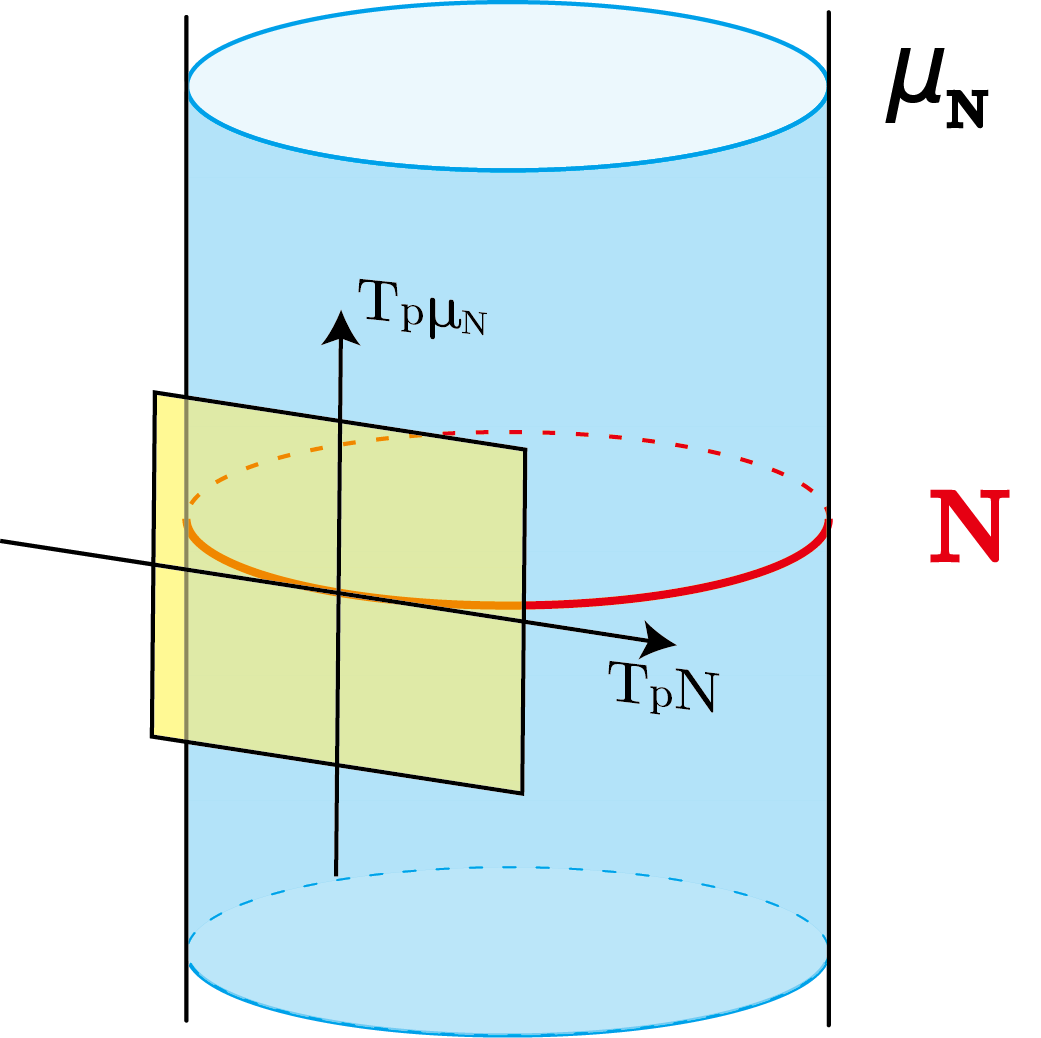
\includegraphics[width=0.4\textwidth]{figures/figure11.png}\\
	\caption{}
	\label{fig6}
\end{figure}
For $p \in N$, we consider the differential
$$\textstyle d(\exp|_W)_p:T_p \mu_N \cong \mu_N \bigoplus T_pN = T_pM \longrightarrow T_pM$$
which is the identity. So there exists an invariant open neighbourhood $V$ of $N$ in $W$ such that the smooth map $exp:V \rightarrow M$ is an immersion.

\subsection*{\underline{Step3}} Shrink $V$ to $U$ such that the exponential map maps an invariant neighborhood $U$ of $N$ in $TN^{\perp}$ diffeomorphically onto a
neighborhood of $N$ in $M$.

First we can shrink $V$ to $\tilde{U}$ such that $\exp^{-1}(N) \bigcap \tilde{U}=N$. (Because $N$ is closed, one can choose an open set $\tilde{U}_p$ near each point $p$ of $N$ which satisfies $\exp^{-1}(N) \bigcap \tilde{U}_p \subseteq N$, then take $\tilde{U}:=\bigcup_{p \in N, g\in G}g\cdot\tilde{U}_p$)

Then
\begin{itemize}
	\item $\exp|_{\tilde{U}}:\tilde{U}\rightarrow M$ is a smooth map that is one-to-one on $N$;
	\item $\exp|_{\tilde{U}}$ maps $N$ diffeomorphically onto $\exp|_{\tilde{U}}(N)$;
	\item $d(\exp|_{\tilde{U}})_p: T_p\mu_N \cong T_pM \rightarrow T_pM$ is identity, thus a linear diffeomorphism for any $p \in N$.
\end{itemize}
So by the \cite{ZW1} (Lecture 10, Theorem 1.4), $\exp$ maps an invariant neighborhood $U$ of $N$ in $TN^{\perp}$ diffeomorphically onto a
neighborhood of $N$ in $M$.

Until now we have gotten a good idendification between the open invariant neighborhood $U$ of $N$ in $\mu_N$ and a neighborhood of $N$ in $M$. Now all we need is to construct a good idendification between $\mu_N$ and the open tubular neighbourhood.
\subsection*{\underline{Step4}} Define some functions to shrink $TN^{\perp}$ into $U$.

Define the function
$f:N \rightarrow \mathbb{R}$ by
$f(p) = \sup\{r\mid B_r(p) \cap \mu_N \subseteq U\} $. Then 
\begin{itemize}
	\item $f(g\cdot p)=f(p)$ for any $p \in N, g \in G$\label{item:sym}
	\item $f$ is a lower semicontinuous positive function on $N$, i.e.
	$$\varliminf_{x\rightarrow p \text{ in } N}f(x) \geqslant f(p) \qquad \text{ for any }p \in N$$
\end{itemize}
By the method of P.O.U. (c.f. Lecture 4 in \cite{ZW1}) we can show that there exists a smooth function $h$ on $N$ with
$$0<h(p)<f(p) \qquad \text{ for any }p \in N$$
This function has better properties then the original function. However, it does not satisfy the equality $h(g\cdot p)=h(p)$. It doesn't matter because we can takes the ``average function" by
\begin{equation}
\begin{aligned}
	k:N&\longrightarrow\hspace{1cm} \mathbb{R}\\
	p\;&\mapsto \frac{1}{|G|}\sum_{g \in G} h(g \cdot p)
	\label{eq:aver}
\end{aligned}
\end{equation}
then $$0<k(p)=\frac{1}{|G|}\sum_{g \in G} h(g \cdot p)<\frac{1}{|G|}\sum_{g \in G} f(g \cdot p)=f(p)$$
and $$k(g\cdot p)=k(p)\qquad \text{ for any }g \in G$$

\subsection*{\underline{Step5}}
Now define $\pi:\mu_N \rightarrow N$ to be the projection, and 
\begin{equation*}
\begin{aligned}
\phi:\mu_N&\longrightarrow\hspace{0.5cm} \mu_N\\
v\;&\mapsto \frac{k(\pi(v)) \, v}{\sqrt{1+\left<v,v\right>}}
\end{aligned}
\end{equation*}
Then $\varphi$ is an equivariant diffeomorphism
onto its image, which is the open set $$\{v \in \mu_N \big|\; |v|<k(\pi(v))\}$$
And $\Phi\!:=\!\exp \circ\, \varphi$ is the required equivarient map from the normal bundle $\mu_N$ onto an open neighborhood of $N$ in $M$, which is the identity map when restricted to $N$.

\begin{figure}[th]
	\centering
	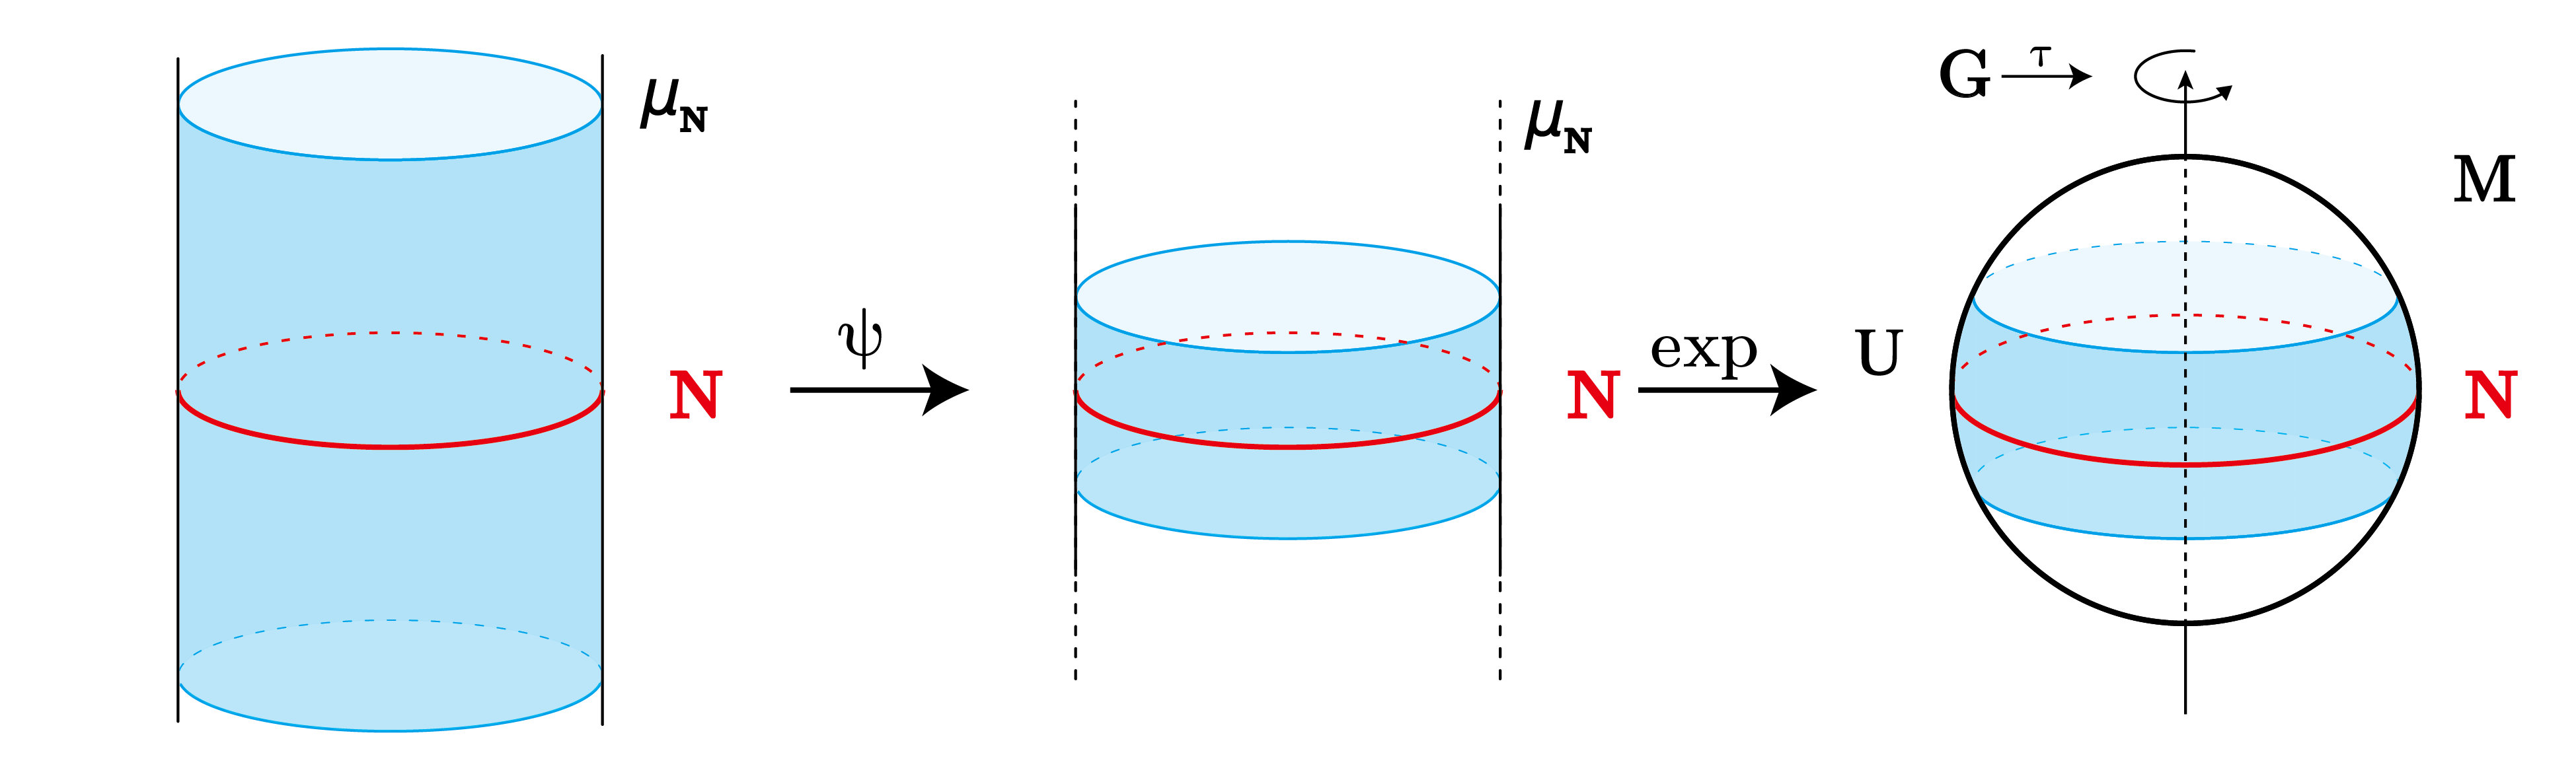
\includegraphics[width=\textwidth]{figures/final3.png}\\
	\caption{}
	\label{fig5}
\end{figure}
\section{From Finite to Compact}
Now we need to prove the main theorem \textbf{Theorem \ref{thm:main}}.

By staring at the proof when $G$ is finite, one can see the finite condition is only used in the formula (\ref{eq:riemet}) and (\ref{eq:aver}). So, to prove the theorem when $G$ is compact, we only need:
\begin{itemize}
	\item  Construct an $G$-invarient Riemannian metric $\{-,-\}$ from a common Riemannian metric
	$\left<-,-\right>$.
	\item Redefine the ``average function" $k(x)$ from $h(x)$.
\end{itemize}
To solve these problems, one needs to calculate the ``average" of the function, or ``integrate a function on $G$ ". So we need a good volume form on $G$ which is compatible with the group structures. (Notice that the Lie group is always compatible)
\begin{defn}(The left invariant volume form)
	A volume form $\omega$ on a Lie group $G$ is called \textbf{left invariant} if $L_g^*\omega=\omega$ for any $g \in G$.
	Sometimes we denoted the left invariant volume form by $\,d\mu_G$.
\end{defn}
\begin{theorem}(The Existence of the left invariant volume form)
	Suppose $G$ is a Lie group. Then there exists a left invariant volume form on $G$.
\end{theorem}
\begin{proof}
	Take the nonzero element $\omega_e \in \wedge^nT_e^*G$, then define an n-form $\omega$ on $G$ by letting $\omega_g= L_{g^{-1}}^*\omega_e$. One can check this is indeed a vvvariant volume form.
\end{proof}
\begin{remark}
	We assume that $\omega$ is positive with respect to the orientation of $G$, and we denote
	$$|G|:=\int_G \,d\mu_G$$
	to be the volumn of the Lie group $G$ when $G$ is compact.
\end{remark}
Now we can define a new Riemannian metric $\{-,-\}$ on $M$ by using the technique of ``averaging over the group":
\begin{equation}
\{v,w\}_m=\frac{1}{|G|}\int_G \left<g \cdot v,g\cdot w\right>_{g\cdot m}\,d\mu_G
\label{eq:riemet2}
\end{equation}
We will check that $\{-,-\}$ is invariant:
\begin{equation*}
\begin{aligned}
\{h \cdot v,h \cdot w\}_{h \cdot m}=&\frac{1}{|G|}\int_G \left<gh \cdot v,gh\cdot w\right>_{gh\cdot m}\,d\mu_G\\
=&\frac{1}{|G|}\int_G \left<g \cdot v,g\cdot w\right>_{g\cdot m}\,d\mu_G=\{v,w\}_{m}
\end{aligned}
\end{equation*}
We can also fix the formula (\ref{eq:aver}) by
\begin{equation}
\begin{aligned}
k:N&\longrightarrow\hspace{1.1cm} \mathbb{R}\\
p\;&\mapsto \frac{1}{|G|}\int_G h(g \cdot p)\,d\mu_G
\label{eq:aver2}
\end{aligned}
\end{equation}
then one can find out
$$0<k(p)=\frac{1}{|G|}\int_G h(g \cdot p)\,d\mu_G<\frac{1}{|G|}\int_G f(g \cdot p)\,d\mu_G=f(p)$$
and $$k(g\cdot p)=k(p)\qquad \text{ for any }g \in G$$
thus we have proved the case when $G$ is compact.

\section{From Compact to Proper} 
Now we want to remove the ``compactness" assumption. We have the following generalized theorem:
\begin{theorem}(The Generalized Equivariant Tubular Neighborhood Theorem)
	\label{thm:equi2}
	Suppose a Lie group $G$
	acts on a smooth manifold $M$ \textbf{properly}. Then for any $G$-invariant smooth submanifold $N$
	of $M$, there exists a $G$-equivariant diffeomorphism from the normal bundle $\mu_N$ of $N$ to a
	neighborhood of $N$ in $M$, which is the identity map when restricted to $N$.
\end{theorem}
\begin{remark}\
\begin{itemize}
	\item We still have left invariant volume form, but the integral in (\ref{eq:riemet2}) and (\ref{eq:aver2}) may diverge. So in the proof, we will add a ``potential item" to force the integral to converge, which uses the ``proper" assumption.
	\item If we remove the ``proper" assumption, the theorem may fail when we consider the following example:
\end{itemize}
\end{remark}
\begin{eg}
	Suppose $G=\mathbb{R}^+$ acts on $M=\mathbb{R}^2$ by multiplying, and $N=\{(x,0) \in \mathbb{R}\}$ to be the embedding submanifold of $M$. Then one cannot find an equivariant tubular neighborhood because there is no ``slice" of $(0,0)$. (See Figure \ref{fig7}) Also the action is non-proper because
	$$\mathcal{A}^{-1}([-1,1] \times [-1,1])=\mathbb{R}^+ \times [-1,1]$$
	is  non-compact.
\end{eg}
\begin{figure}[th]
	\centering
	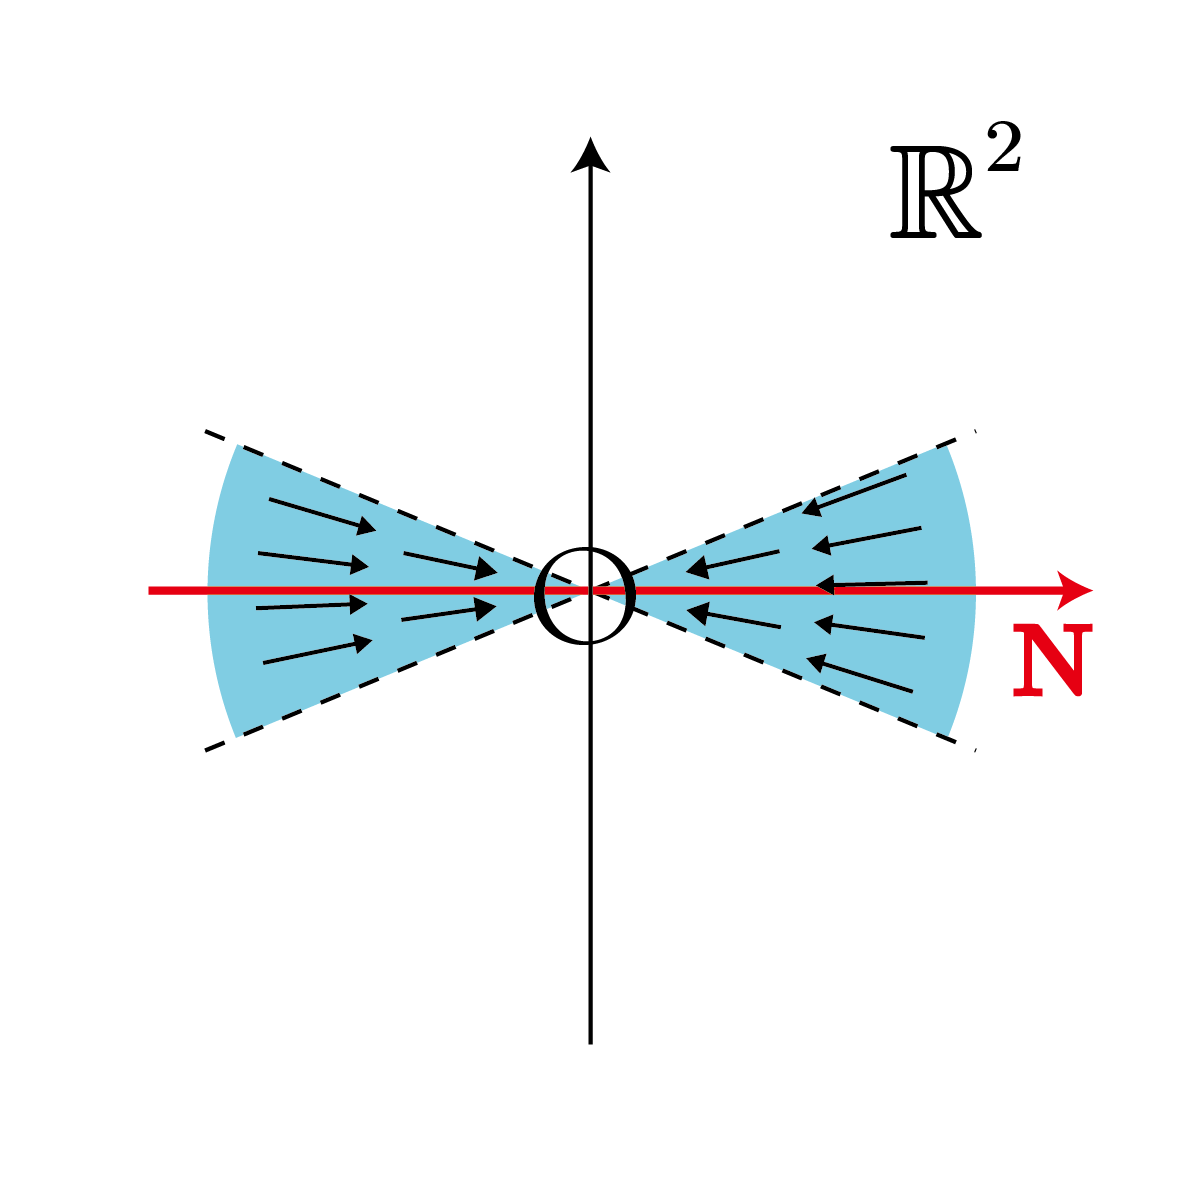
\includegraphics[width=0.4\textwidth]{figures/final4-01.png}\\
	\caption{}
	\label{fig7}
\end{figure}
Roughly speaking, the ``proper" condition is the generalization of the ``compactness" condition. We will find an equivalent description which will contribute to our proof. Before that, let us see an example:
\begin{eg}
	\label{eg:z}
	When $G=\mathbb{Z}$, then the $\mathbb{Z}$-action is proper
\begin{flalign*}
\Leftrightarrow&\mathcal{A}:\mathbb{Z}\times M \rightarrow M \times M \text{ is proper }\\
\Leftrightarrow& U_1, U_2 \subseteq M,\; \#\{g \in \mathbb{Z} \mid gU_1 \cap U_2 \neq \varnothing\} \text{ is finite}\\
\Leftrightarrow& \forall\, m \in M, \exists \text{ a neighbourhood } U_m \text{ of } m \text{ in } M;\\
& \forall\, m_0 \in M, \exists \text{ a neighbourhood } U_{m_0} \text{ of } m_0 \text{ in } M, \text{ such that}\\
& \hspace{1.2cm}\{g \in \mathbb{Z} \mid gU_m \cap U_{m_0} \neq \varnothing\}\hspace{0.5cm}\text{ is finite}
\end{flalign*}
\end{eg}
Suppose $U,V \subseteq M$, and denote
$$U \triangle_GV=\{g \in G \mid gU \cap V \neq \varnothing\}$$
\begin{defn}
	$U$ is \textbf{thin relative to} $V$ if $\widebar{U \triangle_GV}$ is compact in $G$. 
\end{defn}
\begin{remark}
	$U$ is thin relative to $V$ if and only if $V$ is thin relative to $U$ because $gU \cap V=g(g^{-1}V \cap U)$.
\end{remark}
\begin{defn}
	Suppose $U \subseteq M$. We call $U$ a \textbf{small subset} of $M$ if for any $m \in M$, there exists a neighbourhood $U_m$ of $m$ in $M$ which is thin relative to $U$.
\end{defn}
\begin{proposition}
	Suppose the Lie group $G$ acts on a smooth manifold $M$ properly. Then any $m \in M$ has a small neighbourhood.
\end{proposition}
\begin{proof}
	One can prove this from the definition. You can refer to \textbf{Example \ref{eg:z}}.
\end{proof}
\begin{defn}
	Suppose the Lie group $G$ acts on a smooth manifold $M$ properly. We call $F \subseteq M$ a \textbf{converge set}\footnote{In reference, this set is called ``the fat closed fundamental set".} if $F$ is small, closed subset of $M$, and $G (F^{\circ})=M$ where $F^{\circ}$ denotes the interior of $F$.
\end{defn}
Using the technique in \cite{ZW1}(Lecture 4, Lemma 1.3), one can prove that a proper smooth $G$-manifold always has a converge set. For a concrete proof, see \cite{RS}(Lemma 3.6).
\begin{proof}\textit{of the Theorem \ref{thm:equi2}}. Let $F$ be a converge set in $M$. Let $\left<-,-\right>$ be a common Riemannian metric on $M$. By P.O.U, there exist a smooth map $\alpha:M\rightarrow [0,\infty)$ such that
	\begin{itemize}
		\item $\supp \alpha \subseteq F^{\circ}$
		\item $\alpha$ is not identically zero on any $G$-orbit.
	\end{itemize}
define 
\begin{equation}
\{v,w\}_m=\frac{1}{|G|}\int_G \alpha(g\cdot m) \left<g \cdot v,g\cdot w\right>_{g\cdot m}\,d\mu_G
\label{eq:riemet3}
\end{equation}
The right hand side converges because
$$\alpha(g \cdot x)=0 \qquad\text{ for any } g \notin \widebar{\{x\} \triangle_GF}$$
$\{v,w\}_m$ is smooth at $m_0$ because exists a small neighbourhood $U_{m_0}$ such that 
$$\alpha(g \cdot x)=0 \qquad\text{ for any } x \in U_{m_0},\;\; g \notin \widebar{U_{m
	_0} \triangle_GF}$$
$$\Rightarrow \{v,w\}\Big|_{U_{m_0}}=\frac{1}{|G|}\int_{\overline{U_{m_0} \triangle_GF}} \alpha(g\cdot m) \left<g \cdot v,g\cdot w\right>_{g\cdot m}\,d\mu_G$$
Naturally $\{-,-\}_p$ is symmetric, positive definite and $G$-invariant.\\

Now we define $k(x)$ by 
\begin{equation}
\begin{aligned}
k:N&\longrightarrow\hspace{1.4cm} \mathbb{R}\\
p\;&\mapsto \frac{\int_G  \alpha (g \cdot p) h(g \cdot p)\,d\mu_G}{\int_G  \alpha (g \cdot p) \,d\mu_G}
\label{eq:aver3}
\end{aligned}
\end{equation}
Using the same method one can find out that $k(p)$ is well-defined and smooth. Moreover,
$$0<k(p)=\frac{\int_G  \alpha (g \cdot p) h(g \cdot p)\,d\mu_G}{\int_G  \alpha (g \cdot p) \,d\mu_G}<\frac{\int_G  \alpha (g \cdot p) f(g \cdot p)\,d\mu_G}{\int_G  \alpha (g \cdot p) \,d\mu_G}=f(p)$$
and $$k(g\cdot p)=k(p)\qquad \text{ for any }g \in G$$
Thus the proof is completed.
\end{proof}
\section{Miscellaneous} 
At last, I want to give special thank to the Prof.Shentu for his generous help, without whom I cannot take the finite group as the first case.
%%%%%%%%%%%%%%%%%%%%%%%%%%%%%%%%%%%%%%%%%%%%%%%%%%%%%%%%%%%%%%%%%%%%%%%%%%%%%%%%%%%%%%%%%%%%%

 
   


%%%%%%%%%%%%%%%%%%%%%%%%%%%%%%%%%%%%%%%%%%%%%%%%%%%%%%%%%%%%%%%%%%%%%%%%%%

 




%%%%%%%%%%%%%%%%%%%%%%%%%%%%%%%%%%%%%%%%%%%%%%%%%%%%%%%%%%%%%%%%%%%%%%%%%%%%%%%%%%%%%%%%%%%%%%%




\begin{thebibliography}{99}

 
%\bibitem{AF12}%
%Antunes, P., Freitas, P.: Optimal spectral rectangles and lattice ellipses. \emph{Proc. Royal Soc. London Ser. A.} \textbf{469} (2012), 20120492.
\bibitem{ZW1}
Zuoqin Wang. \emph{Differential Manifold}. 2018. url:http://staff.ustc.edu.cn/$\sim$wangzuoq/Courses/18F-Manifolds/index.html
\bibitem{ZW2}
Zuoqin Wang. \emph{Riemannian Geometry}. 2016. url:http://staff.ustc.edu.cn/$\sim$wangzuoq/Courses/16S-RiemGeom/index.html
\bibitem{HSD}
Hurder S, Toben D. \emph{The equivariant LS-category of polar actions}[J]. Topology and its Applications, 2009, 156(3): 500-514.
\bibitem{GB}
G. Bredon, \emph{Introduction to compact transformation groups}, Vol. 46, Academic Press, New York, 1972.
\bibitem{PGA}
Kankaanrinta M. \emph{Equivariant collaring, tubular neighbourhood and gluing theorems for proper Lie group actions}[J]. Algebraic \& Geometric Topology, 2007, 7(1): 1-27.
\bibitem{RS}
R. S. Palais, \emph{On the existence of slices for actions of non-compact Lie groups}, Ann. of
Math.(2) 73 (1961) 295--323
\bibitem{JJ}
John W. Milnor and James D. Stashe↵. \emph{Characteristic
Classes}. Annals of Math. Series, No. 76.
Princeton University Press, first edition, 1974.
  

\end{thebibliography}


\end{document}




